\section{Software Architecture}
This chapter describes the architecture of the software developed. First there will be a description of the big picture of the software, which shows the separation the into different parts. Each of these parts will then be explained in greater detail in a separate chapter.

The software architecture has to fulfil multiple requirements for this project. It should be easily extendable with new algorithms and \acrshort{acro:UI} extensions. The input and output format of the application should be independent from the algorithms to support different file types like bitmap images or \gls{gloss:DXF}/\gls{gloss:DWG} formats. The algorithms of the application should be linked together as workflows which then can be executed by an engine simultaneously.

The idea behind this separation concept is that it should be possible to create new combinations of algorithm pipelines with already implemented algorithms. Every algorithm is just a blackbox which can be connected together with other algorithms to create a processing pipeline, called workflow. This makes it possible to replace existing algorithms and test out new ideas without modifying other parts of the pipeline. 

\begin{figure}[h]
  \centering
      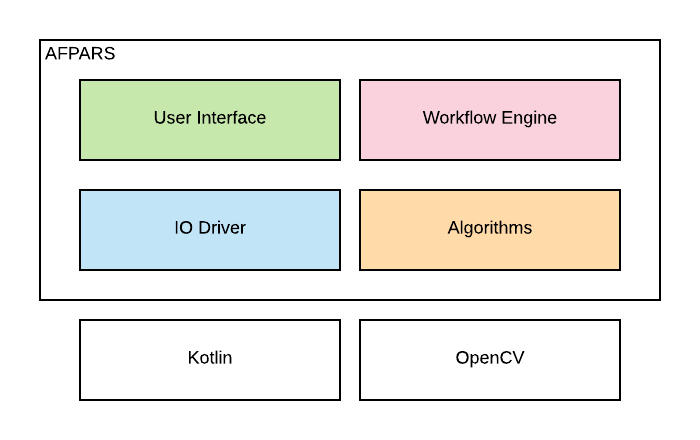
\includegraphics[width=1\textwidth]{AFPARS_Architecture}
  \caption{AFPARS software architecture.}
  \label{fig:AFPARS_Architecture}
\end{figure}


To fulfil these requirements, the architecture of the software is split into four parts as shown in figure \ref{fig:AFPARS_Architecture}. The complete application is based on the \acrfull{acro:JVM} where \gls{gloss:Kotlin} is running on. For image processing and recognition the application uses the library \gls{gloss:OpenCV}.

Every part of the architecture has its own area of responsibility and is connected with the other parts through interfaces which have been designed to be as generic as possible to support the most flexibility.

\subsection{Programming Language}

The software is built with the modern language \gls{gloss:Kotlin}, which is a statically typed programming language for the \acrfull{acro:JVM}. It supports special language features like extension methods, optional parameters and functional programming concepts, which all were used in this project and help to make the code more readable and maintainable \citep{kotlin}.

\subsubsection{Extension Methods}
This section shows an example how the new language is used in the software.

The language feature \flqq Extension Methods\frqq  can be used to make the code more readable. It extends an existing object with a new method without the concept of inheritance. The code of the method will be outsourced into a separate file.

\begin{lstlisting}[caption={Erode image without extension methods},label={lst:imageOperations},language=Java]
// threshold image
Imgproc.threshold(image, image, 128.0, 255.0, 
		Imgproc.THRESH_BINARY)

// erode image
val structureSize = 3
val element = Imgproc.getStructuringElement(Imgproc.MORPH_RECT, 
        Size(structureSize.toDouble(), structureSize.toDouble()))
Imgproc.erode(image, image, element)
\end{lstlisting}

It is used in this software to make calls to \gls{gloss:OpenCV} more natural for object oriented developers. For example instead of using the static Imgproc class (Listing \ref{lst:imageOperations}), it is possible to call a lot of methods on the Mat object itself (Listing \ref{lst:imageOperationsWithExtensions}).

\begin{lstlisting}[caption={Erode image with extension methods},label={lst:imageOperationsWithExtensions},language=Java]
// threshold image
image.threshold(128.0, 255.0, Imgproc.THRESH_BINARY)

// erode image
image.erode(3)
\end{lstlisting}

\pagebreak

\subsection{Meta Format}
To support the different input and output formats the architecture uses a meta format for the
floor plan images called AFImage. Different \gls{gloss:Drivers} add the support for multiple file formats. With this architecture it is possible to extend the software with new file formats and work internally with the meta container format.

\begin{figure}[h]
  \centering
      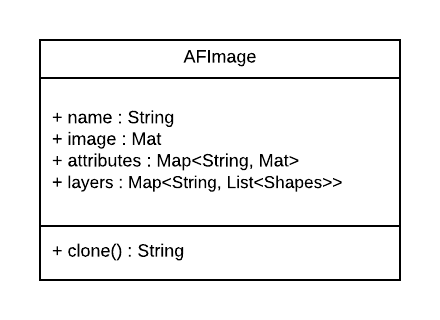
\includegraphics[width=0.6\textwidth]{AFImage_CD}
  \caption{AFImage class diagram.}
  \label{fig:AFImage_CD}
\end{figure}

The meta container AFImage contains a map of attributes (Figure \ref{fig:AFImage_CD}) which can be used by algorithms to get information created by other algorithms or to store information into an existing image.

To interact with the user interface there is also a map of layers which contains shapes that are printed onto the image. The software uses this for example for recognised doors or rooms which are shown as overlay.

By default there is an attribute called "originalimage" which is a copy of the original image read by the AFImageReader. This is used in some algorithms to have access to the original, unprocessed picture.

\pagebreak

\subsection{Input \& Output}
The following sections gives a brief overview about the different input and output formats used by the software.

\subsubsection{Raster Graphics}
For importing floor-plans into the software the decision was made to only read raster graphics like JPEG or PNG file formats. Raster graphics are flat pixel based images like pictures captured by a photo-camera.

The disadvantage of this restriction is that raster images do not contain any layers or information about objects of the floor-plan. Usually floor-plans are stored in a \gls{gloss:DXF} or \gls{gloss:DWG} file format and contain different layers with multiple objects which could be used to simply detect doors and walls and other steps which are done in the semantic analysis.

\begin{figure}[h]
	\centering
	\subfloat[Layers of 50er EG.]{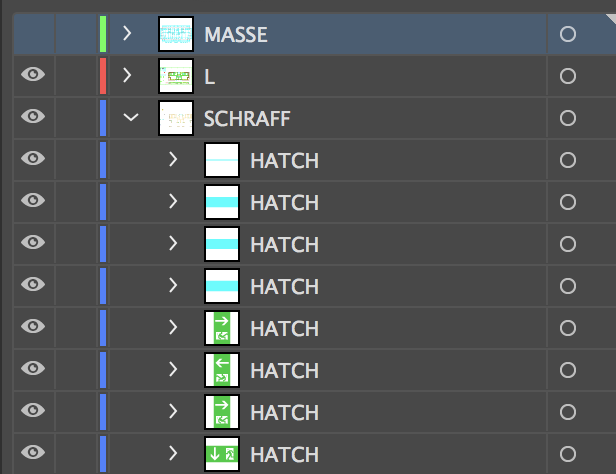
\includegraphics[width=0.3\textwidth]{layers_50er_eg}\label{fig:layers_50_er_eg}}
	\hfill
	\subfloat[Layers of A N1.]{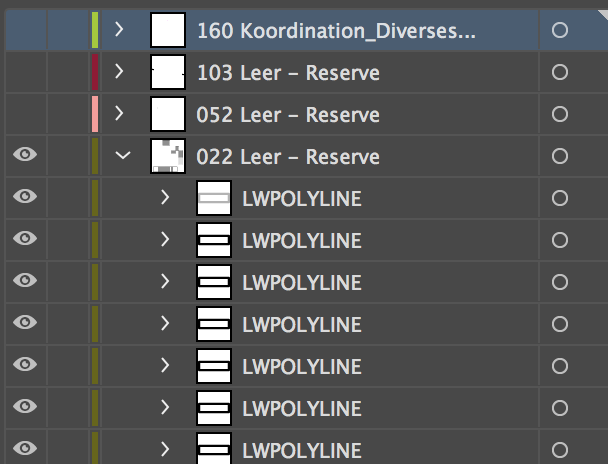
\includegraphics[width=0.3\textwidth]{layers_a_n1}\label{fig:layers_a_n1}}
	\hfill
	\subfloat[Layers of OG.]{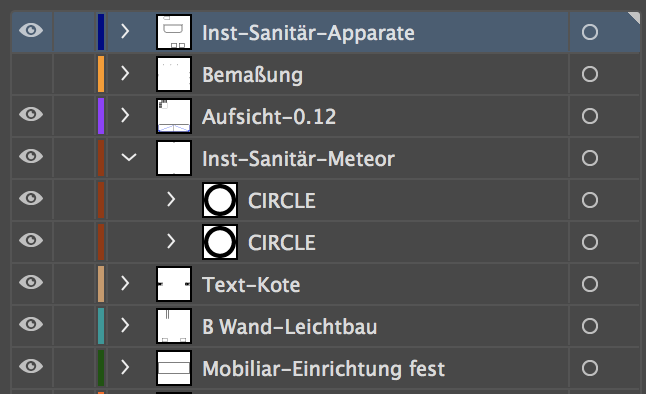
\includegraphics[width=0.3\textwidth]{layers_og}\label{fig:layers_og}}
	\caption{Layers of different DWG floor-plans. }
	\label{fig:layer_comparison}
\end{figure}

As figure \ref{fig:layer_comparison} shows, there is no convention or standard for the layer structure of a \gls{gloss:DXF} or \gls{gloss:DWG} file. This problem lead to the decision to not work with vector based graphics formats as input and only work with raster images of floor-plans.

The advantage of working with raster graphics is that the software is able to use conventional methods for image processing like pixel based filters.

\subsubsection{DWG / DXF}
As requested by the client, the software should support the import and export of DWG and DXF formats. These file formats are standard in the architectural environment and can be imported and exported by the software AutoCAD of the company Autodesk.

There are several libraries for Java which support reading and writing of DWG and DXF files, but a lot of them are not maintained anymore or cost something. The table \ref{tbl:DWGEvaluationResult} shows the evaluated libraries together with the reason, why they are not suitable for this software (Please consult table \ref{tbl:DWGEvaluationMatrix} in the appendix for an extended comparison).

\begin{table}[h]
\centering
\caption{DWG / DXF evaluation result.}
\label{tbl:DWGEvaluationResult}
\begin{tabular}{@{}lll@{}}
\toprule
Name         & Vendor         & Reason                                               \\ \midrule
YCAD Library & Ed Karlo       & No documentation and very unintuitive.                \\
Teigha       & ODA            & Too expensive and only for conversion.               \\
Kabeja       & -              & Could not read the example document.                 \\
Tika         & Apache         & Only a meta text reader.                             \\
jnetcad      & Johannes Raida & Only a converter.                                    \\
CaffViewer   & DeCaff         & Too expensive but able to read the example document. \\ \bottomrule
\end{tabular}
\end{table}

The only library which could read the test document provided by the client is the CaffViewer. But it is licensed under a closed source license and costs about 1350 Euro.

\subsubsection{Scalable Vector Graphics}
Because DWG and DXF support could not be implemented, rooms and other shapes which the software recognises can be exported to \gls{acro:SVG}.

In contrast to the raster image format, the \gls{acro:SVG} file contains commands to draw the image later. This is useful to resize an image without loss of quality and it is possible to select every single element of image.

With \gls{acro:SVG} it is possible to create an overlay for an existing plan.

\subsubsection{Comma-separated Values}
For exporting the different rooms and their room size, the software contains \gls{acro:CSV} format support. This file format is used to store table data like Microsoft Excel data-sheets.

\pagebreak
\subsection{Algorithm}
The architecture of the algorithms follows the single responsibility principle \citep[p.~484]{mclaughlin_pollice_west_2010}. To simply reuse and replace algorithms in a pipeline, every algorithm is responsible for solving just one problem. For example the morphological transform algorithm just creates a clean image of a given input image and has no other task to do.

\begin{figure}[h]
  \centering
      \includegraphics[width=0.6\textwidth]{IAlgorithm_CD}
  \caption{Algorithm interface class diagram.}
  \label{fig:IAlgorithm_CD}
\end{figure}

An algorithm is context unaware and stateless. It gets an input image and returns an output image which maybe is enhanced by more information or pixel based processed (Figure \ref{fig:IAlgorithm_CD}).

\subsubsection{History}
As seen in figure \ref{fig:IAlgorithm_CD} and figure \ref{fig:parameter_window}, an algorithm is not just able to return one AFImage, instead it can return an unlimited count of AFImages, which then are displayed in the parameter window. These images are used to show a history of the steps the algorithm performed. This makes it easier to set the right parameter for the given algorithm and helps to debug all steps of an algorithm.

\pagebreak
\subsection{Workflow \& Workflow Engine}
To create a pipeline which connects multiple algorithms together, there is the concept of workflows. A workflow is a list of algorithms which have a defined order in which they are executed.

The reason why there is the possibility to define multiple workflows, is to run different combinations of algorithms in parallel or to test out multiple versions of pipelines. With workflows it is also simple to implement a flexible system, where the user is able to create new combinations of algorithms on his own.

\begin{figure}[h]
  \centering
      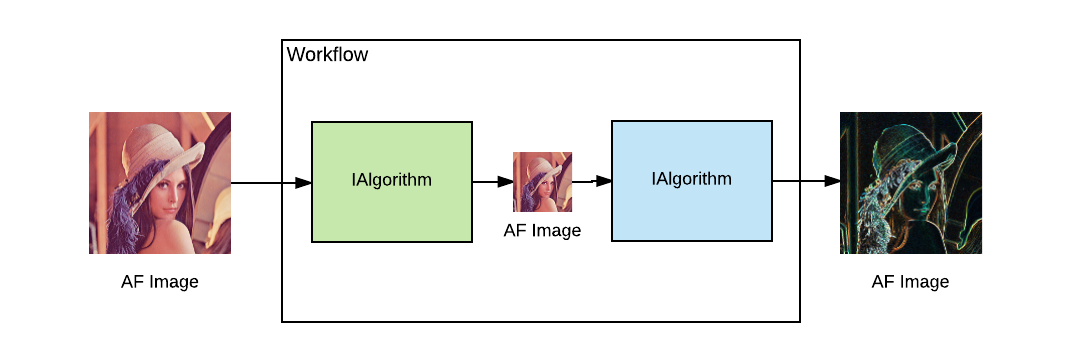
\includegraphics[width=1\textwidth]{workflow}
  \caption{Workflow example with two algorithms.}
  \label{fig:Workflow}
\end{figure}

The execution of a workflow is managed by the workflow engine which takes a workflow and an input image and passed the image through the different algorithms defined in the workflow (Figure \ref{fig:Workflow}).

\begin{figure}[h]
  \centering
      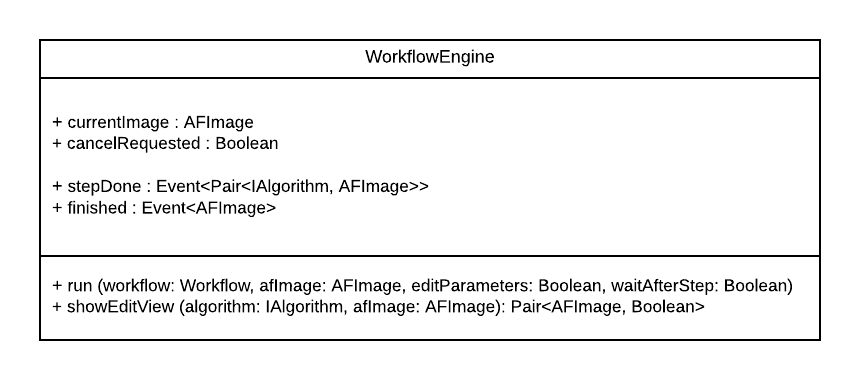
\includegraphics[width=1\textwidth]{WorkflowEngine_CD}
  \caption{Workflow engine class diagram.}
  \label{fig:WorkflowEngine_CD}
\end{figure}

The workflow engine runs the workflows in a new thread and communicates with the application over events. It is possible to stop the workflow after each algorithm and make changes to the current AFImage of the process. This feature is used to let the user fix recognition errors.

It is also possible to show the parameter window which is described in the following chapter (Figure \ref{sub:parameter_window}).

\pagebreak
\subsection{User Interface}

The user interface of the software is designed to be user friendly and very intuitive. It guides the user through the process and offers the tools to fix algorithm errors. The interface itself is very simple and contains only the controls which are absolutely necessarily (Figure \ref{fig:afpars_window}).

\begin{figure}[h!]
  \centering
      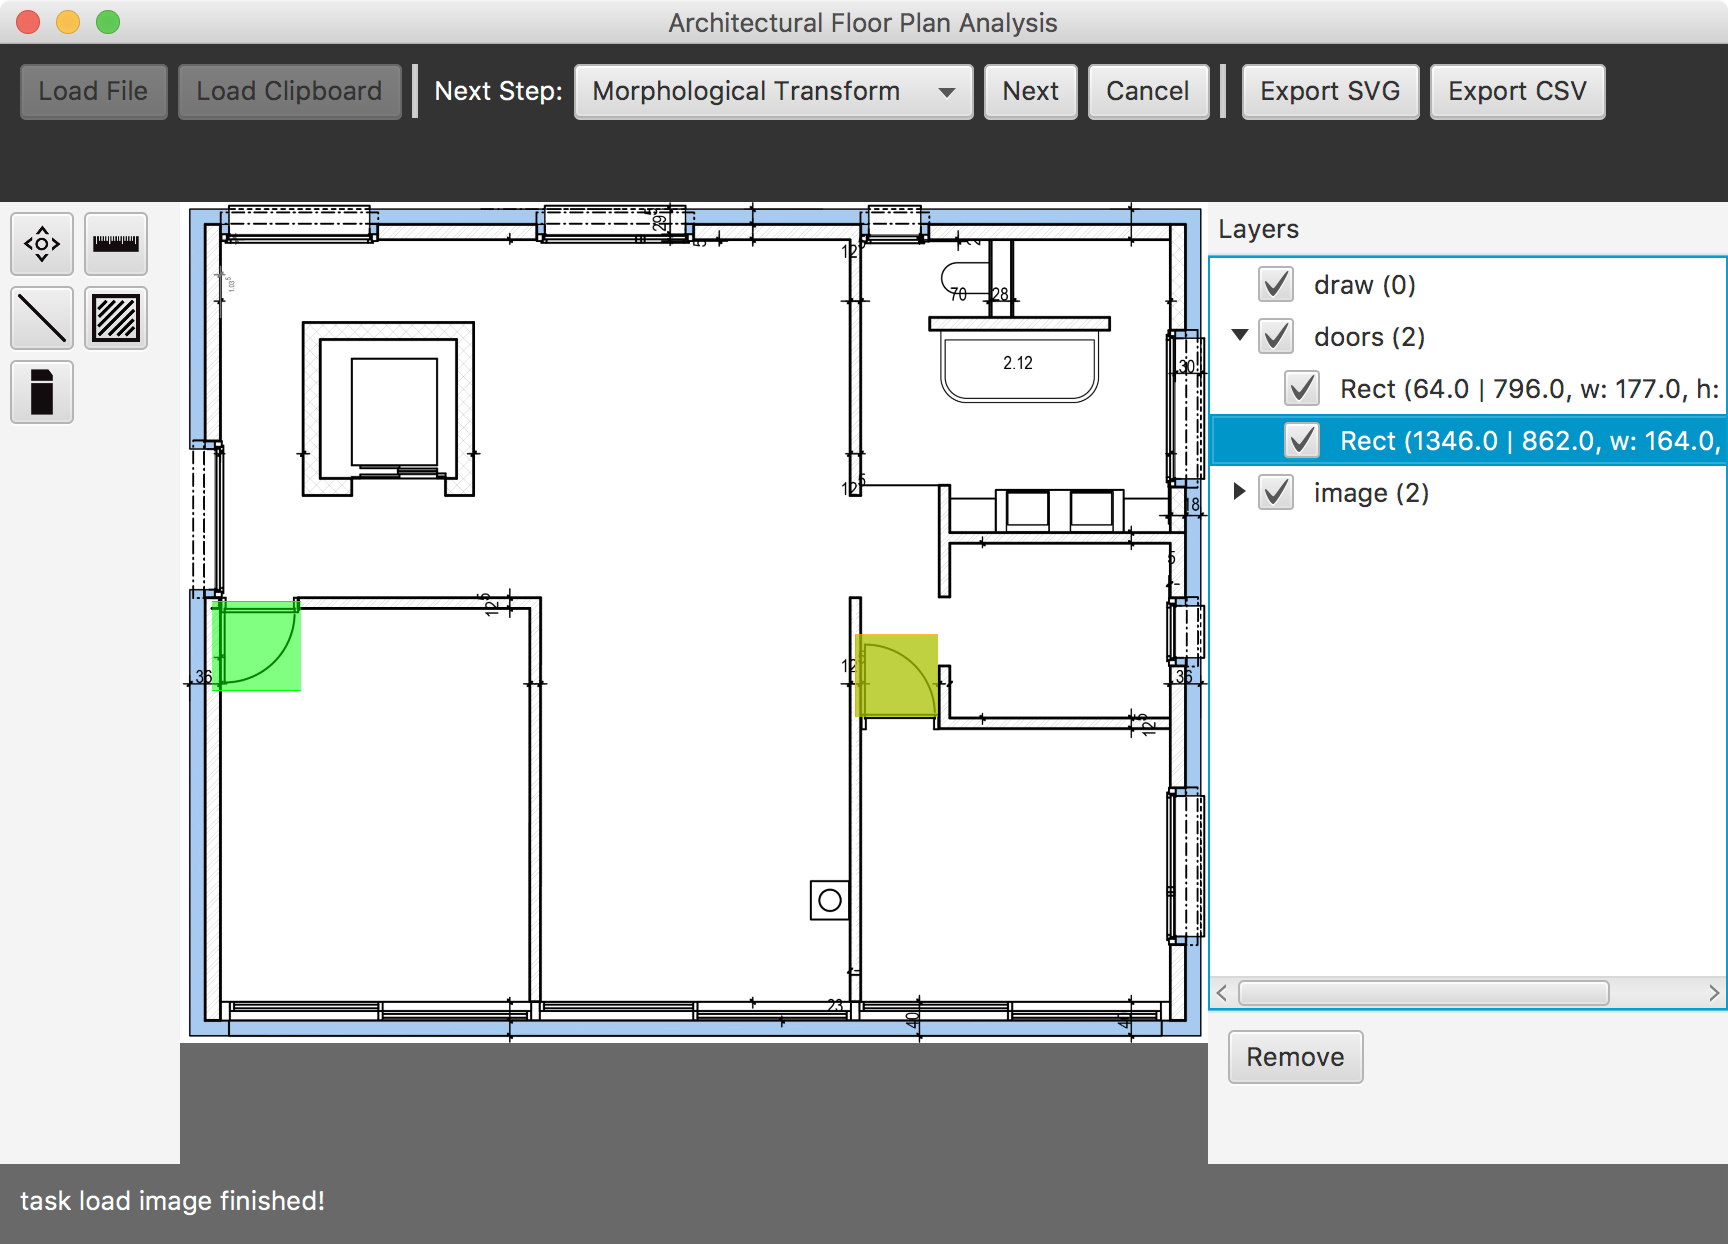
\includegraphics[width=1\textwidth]{afpars_window}
  \caption{Main window of the software.}
  \label{fig:afpars_window}
\end{figure}

\subsubsection{Integration}
\todo{describe why we did not integrate it into another software}

\subsubsection{Layout}

The layout of the interface is inspired by popular design softwares like Adobe Illustrator or Autodesk AutoCAD. The different parts of the layout are shown in figure \ref{fig:afpars_window_zones}.

At the top there is the navigation section which guides the user through the process of the application. The navigation buttons are ordered in a sequential manner to reflect the application workflow. First of all the user has to load the image from a file or the clipboard. After that he is able to start the workflow and run through the different steps.

After finishing the workflow, the user has the possibility to export the different layers or a \gls{acro:CSV} file with all the detected rooms and room sizes.

In the center of the window is the canvas section which is the drawing pane of the application. It always shows the current image of the process and let the user correct and inspect the algorithm output.

To edit the current image, there are tools on the left side of the window. The controls there change the current tool used to manipulate the image.


\begin{figure}[h!]
  \centering
      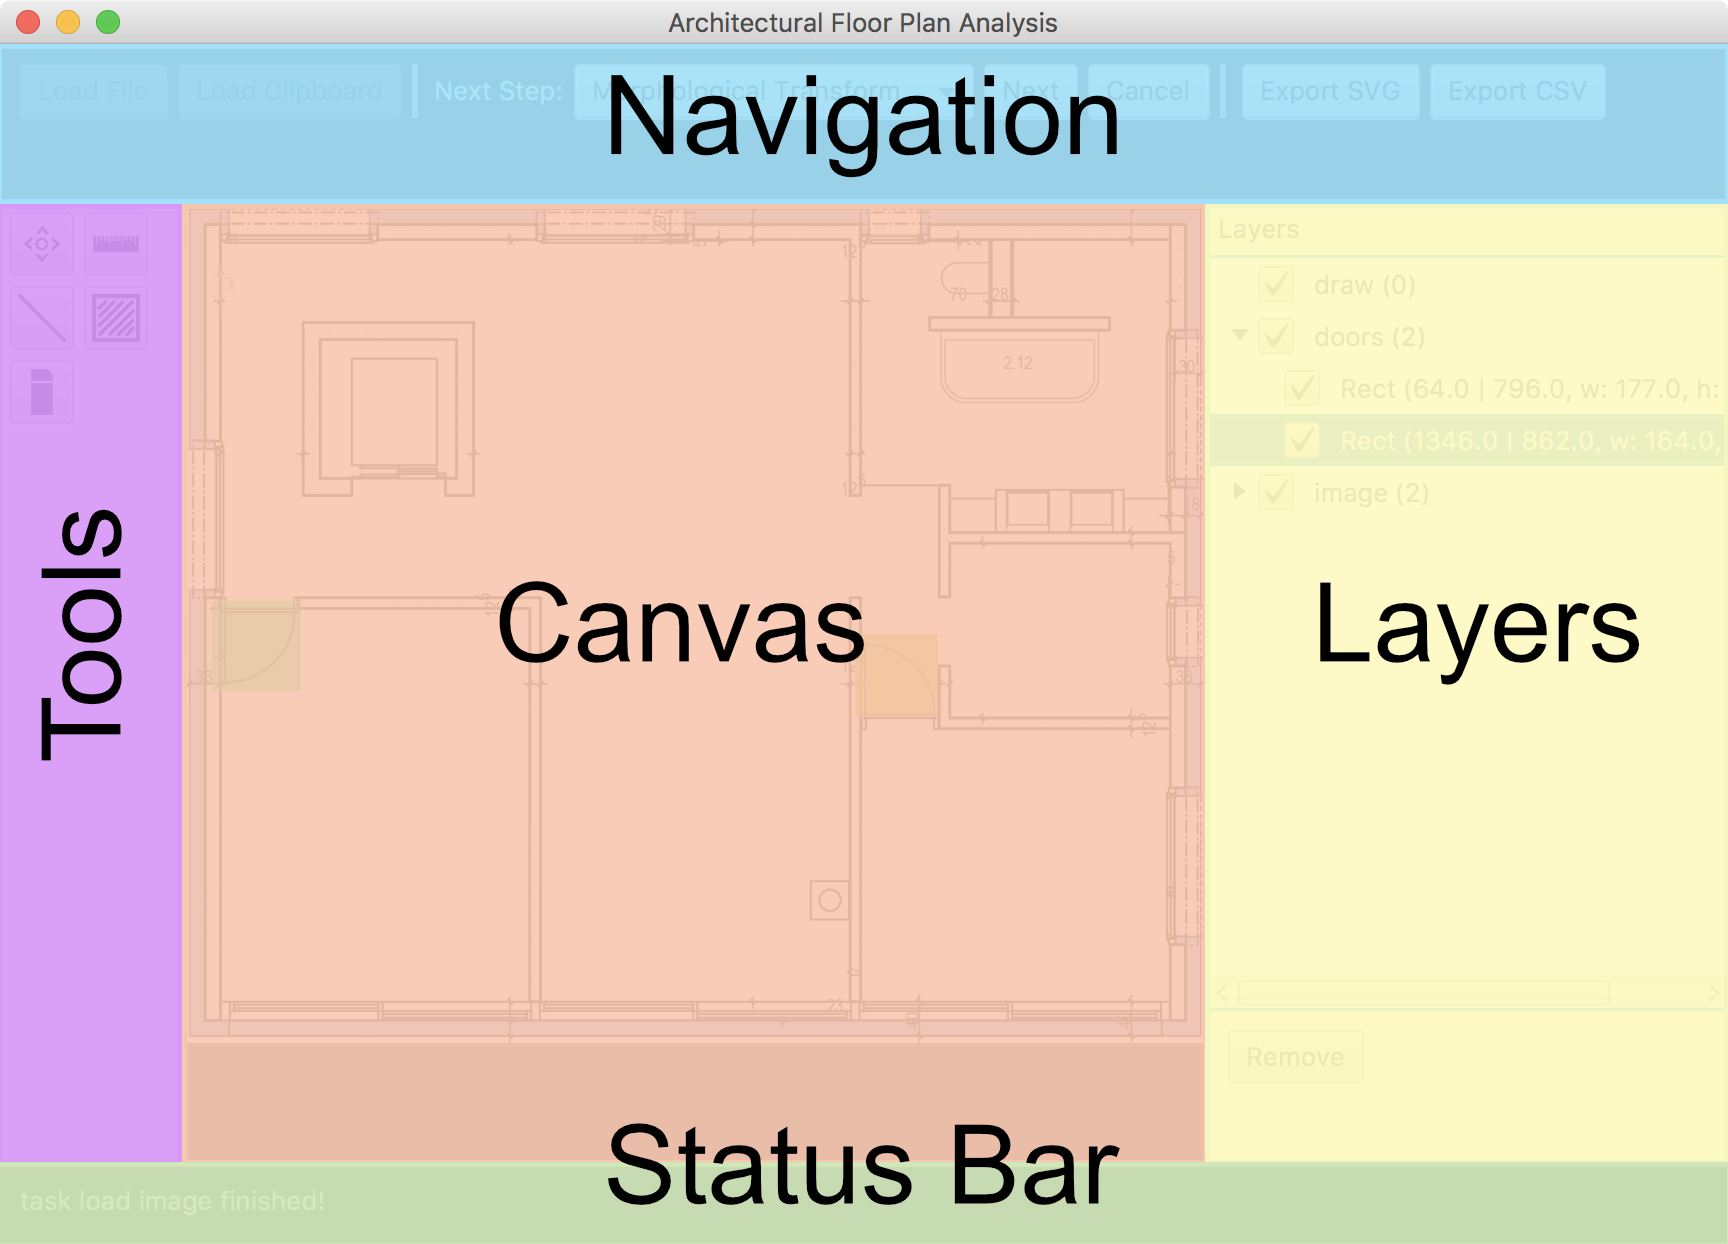
\includegraphics[width=1\textwidth]{afpars_window_zones}
  \caption{Main window with zones.}
  \label{fig:afpars_window_zones}
\end{figure}

On the right side of the application window, there is the layer section. The layer section shows the different layers which are printed onto the canvas. Every layer contains shapes which can be toggled as visible or not. There is always a draw layer which contains all the drawings done by the tools on the right side. It is also possible mark these drawings and to delete them if needed.

Only drawn shapes and detect rooms can be deleted through the user interface. Every other layer is locked and can only be disabled.

At the bottom there is the status bar which shows the status of the different task the user interface is performing.


\subsubsection{Parameter Window} \label{sub:parameter_window}
Because a lot of the algorithms need parameters to set manually, there is the possibility to flag these parameters with an attribute in the code and the software is then able to automatically detect them and show an input field in the user interface. With this input field the user is able to set the parameter or use the default values (Figure \ref{fig:parameter_window}).


\begin{figure}[h!]
  \centering
      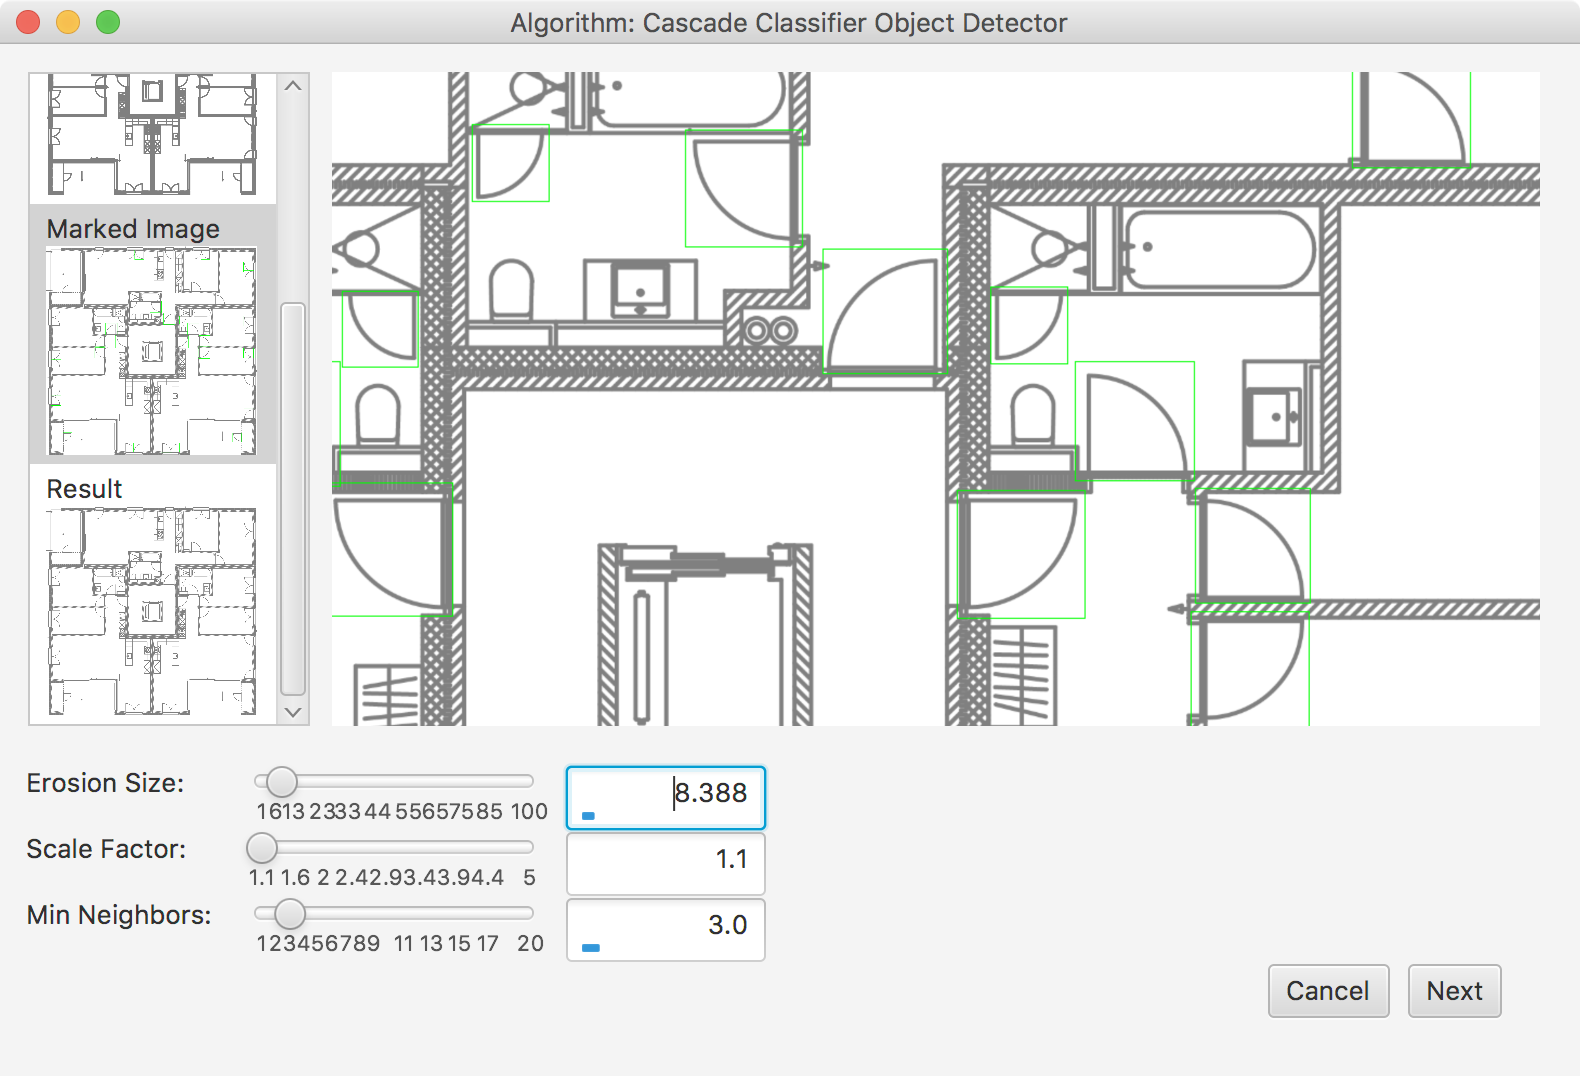
\includegraphics[width=1\textwidth]{parameter_window}
  \caption{Algorithm parameter window.}
  \label{fig:parameter_window}
\end{figure}

This parameter window is shown by the application when an algorithm is started. It runs the algorithm once and then shows the output of it in the preview window. Every change of the parameters let the algorithm run again. With this behaviour the user always gets an instant visual feedback of the changes he made.

\todo{Why it looks like that. (Andere Software)}